\subsection{Flöde vid termisk jämvikt}
\label{sec:steadystatewall}

%To regerenate the figures use /code/pdesolver/generateWallFigApril.m
%with the argument /code/pdesolver/walldata.mat


För att visualisera flödet genom en vägg vid konstant väder och utomhustemperatur görs 
beräkningar med finita elementmetoden och en konstant inomhustemperatur på 
$\unit[20]{^\circ C}$. Utomhusvädret är relativ konstant och är satt till antingen molning 
eller klart och utomhustemperaturen varierar mellan $\unit[6]{^\circ C}$ på natten och 
$\unit[9]{^\circ C}$ på dagen. Detta har gjorts för en vägg utan och en vägg med 
isolering, se figur \ref{fig:energyflow_stst}. Den oisolerade väggen består av 
$\unit[0,5]{m}$ tegel och den isolerade har dessutom $\unit[0,1]{m}$ mineralull. 

\begin{figure}[hpbt]
\centering

\subfloat[Energiflöde ut från insidan av en oisolerad vägg en klar dag.]{
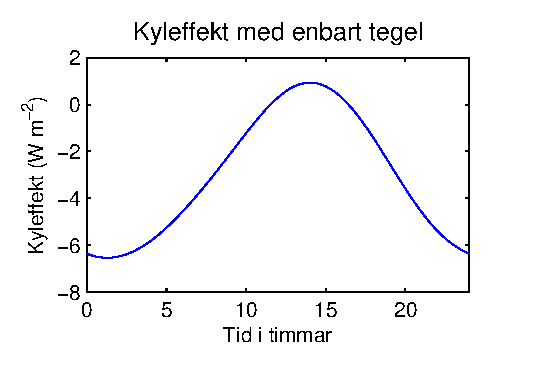
\includegraphics[width=6cm]{images/noinsulationapril.eps}}\vspace{1cm}
\subfloat[Energiflöde ut från insidan av en isolerad vägg en klar dag.]{
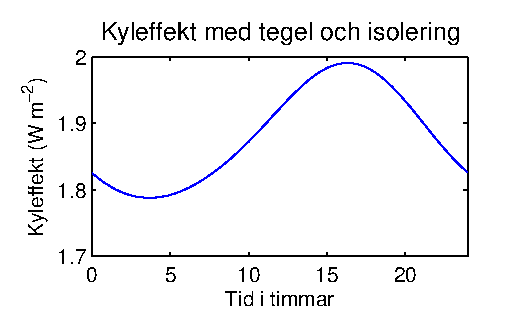
\includegraphics[width=6cm]{images/insulationapril.eps}
}

\subfloat[Energiflöde ut från insidan av en oisoleradvägg en molnig dag.]{
\includegraphics[width=6cm]{images/noinsulationcloud.eps}}\vspace{1cm}
\subfloat[Energiflöde ut från insidan av isolerad vägg en molnig dag.]{
\includegraphics[width=6cm]{images/insulationcloud.eps}
}

\caption{\label{fig:energyflow_stst} Energiflöden ut från insidan av en vägg en dag motsvarande en i mitten av april.
Utomhustemperaturen varierar mellan $\unit[6]{^\circ C}$ på natten och $\unit[9]{^\circ C}$ på dagen. Inomhustemperaturen är satt konstant $\unit[20]{^\circ C}$.}
\end{figure}


%RESULTAT ur graferna 
I figurerna \ref{fig:energyflow_stst} kan vi se att energiflödet genom väggen minskar till 
ungefär en fjärdedel med isolering. Under ett soligt dygn kommer det att flöda värme in i
 fastigheten. På grund av fördröjningen i väggen sker detta främst under natten, 
 och mindre på dagen. Med isolering blir variationen mindre och ett mindre men jämnare 
 energiflöde, under $\unit[1]{W m^{-2}}$, går i fastigheten under hela dygnet.

Under en motsvarande fast molnig dag varierar energiflödet mellan 7 och 10 
$\unit{W m^{-2}}$ till att röra sig mellan 2,1 och 2,3 $\unit{W m^{-2}}$, dock ut ur 
fastigheten. En isolering innebär ett minskat energiutflöde och därmed en minskad 
energiförlust för fastigheten.

Trots att energi flödar in i fastigheten den soliga dygnet så flödar ganska mycket energi 
ut ur fastigheten under det molniga dygnet. Göteborg har 1800 solskenstimmar under ett
 år av de totalt 4380 timmar som solen är över horisonten. Utifrån SMHI:s väderstatistik \cite{SMHIdata}
 kan beräknas att ungefär 37\% av dessa sker under eldningssäsongen, oktober till april. 
 Detta motsvarar ungefär 8\% av dygnets alla timmar. Tyvärr så förlorar fastigheten mer 
 energi än vad den tjänar på att inte isolerat sett till hela eldningssäsongen.

Under en fin sommardag kan det också tänkas att fastigheten värms över den önskade 
temperaturen och energi istället måste läggas på kylning. Med en isolering minskas även 
effekten av detta och energiflödena blir mindre om jämnare.

%%%%%%%%%%%%%%%%%%%%%%%%%%%%%%%%%%%%%%%%%%%%
\paragraph{En molning decemberdag}

Vidare har också energiflödena genom väggen en kall, molnig decemberdag undersökts, 
alltså en dag där energiflödena bör bli ganska stora. Detta kan ses som ett extremfall av
nyår i Göteborg och är då en övre uppskattning på den energiåtgång fastigheten.

 Temperaturen går från $\unit[-5]{^\circ C}$ på dagen till $\unit[-11]{^\circ C}$ 
 Solinstrålningen denna dag är satt till $\unit[20]{\%}$ av vad den skulle varit den den 
 sista december om det varit helt klart. Konvektionskoefficienten har satts till $h=35$ 
 vilket motsvarar en vindhastighet $\unit[5]{m/s}$ parallellt med väggens yta. 
 Beräkningarna är genomförda genom att väggen approximerats med en stav och 
 därefter behandlats med finita elementmetoden.


\begin{figure}[hpbt]
\centering
\subfloat[Energiflöde en  decemberdag från insidan av en oisolerad vägg en molnig dag]{
\includegraphics[width=6cm]{images/noinsulationdec.eps}}\vspace{1cm}
\subfloat[Energiflöde från insidan av en isolerad vägg en molnig dag.]{
\includegraphics[width=6cm]{images/insulationdec.eps}
}
\caption{\label{fig:wall_dec} Energiflöden ut från insidan av en vägg en dag motsvarande en i december.
}
\end{figure}

% Resultat
Även i december blir energiflödet genom en isolerad vägg ungefär en fjädedel av det 
genom en oisolerad dito, se figur \ref{fig:wall_dec}. Här minskar det dock från ungefär 33 
till 7,9 $\unit{W m^{-2}}$ ut ur väggen. Vi ser också i figurerna att energiflödet också blir 
jämnare med isolering – det varierar med mindre än 0,1 $\unit{W m^{-2}}$ över dygnet, 
istället för över 1 $\unit{W m^{-2}}$, utan isolering. Detta är eftersträvansvärt om en jämn inomhustemperatur önskas.


%%%% BURSPRÅK %%%%%%%%%%%%%%%%%%%%%%%%%%%%%%%
\paragraph{Burspråket}

Burspråket är inte uppbyggt av tegel, som de andra väggarna, utan av gips, isolering och koppar på spånskiva, se avsnitt \ref{subsec:walls}. Energiflödet i burspråket visas här för alla tre fallen: solig aprildag, molnig aprildag och molnig decemberdag.

\begin{figure}
\centering
\subfloat[\label{fig:bursprak_april1} Energiflödet från insidan av burspråket en klar aprildag.]{
	\includegraphics[width=6cm]{images/baysunapril.eps}
}
\subfloat[\label{fig:bursprak_april2} Energiflödet från insidan av burspråket en molnig aprildag.]{
	\includegraphics[width=6cm]{images/baynosunapril.eps}
}

\subfloat[\label{fig:bursprak_dec} Energiflödet från insidan av burspråket en molnig decemberdag.]{
	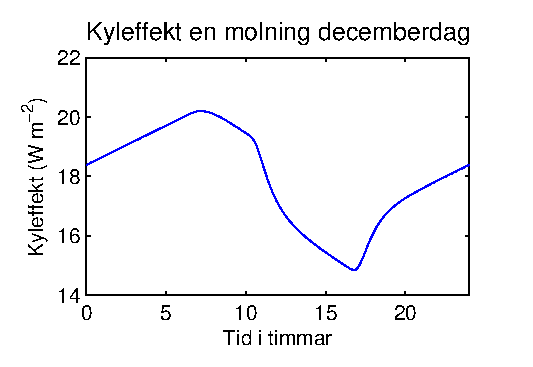
\includegraphics[width=6cm]{images/baynosundec.eps}
}
\caption{\label{fig:bursprak_energi}Energiflödet genom burspråket.}
\end{figure}

Genom burspråket ser energiflödet lite annorlunda ut, figur \ref{fig:bursprak_energi}. En aprilmorgon, innan solen har gått upp, maximeras energiutflödet 10 $\unit{W m^{-2}}$. När solen sedan värmer väggen börjar energi istället flöda in i byggnaden och en riktigt solig dag är det maximala inflödet nästan 20 $\unit{W m^{-2}}$, se figur \ref{fig:bursprak_april1}. En molnig dag stannar det istället på ungefär 1 $\unit{W m^{-2}}$ ut ur väggen, se figur \ref{fig:bursprak_april2}

 En molnig dag  i december är det betydligt kallare och energiutflödet varierar mellan 15 och 20 $\unit{W m^{-2}}$, se figur \ref{fig:bursprak_dec}. En intressant detalj är att kyleffekten på burspråket inte alls är sinusformad, så som flödet genom väggarna i figur \ref{fig:energyflow_stst} och \ref{fig:wall_dec}. Det beror troligen på att väggen är väldigt tunn och reagerar snabbt på olika förändringar.

%%%%%%%%%%%%%%%%%%%%%%%%%%%%%%%%%%%%%%%%%%%%
\paragraph{Temperaturfördelningen utanför väggen}

Även temperaturfödelningen utanför en vägg har beräknats, vilket kan ses i figur \ref{fig:temp_dist}. Det gjordes med finita element metoden applicerad på penaltymetoden.

Temperaturen inne har satts till $\unit[20]{^\circ C}$ och referenstemperaturen ute till 
$\unit[0]{^\circ C}$. Vid fri luft är det ett konvektionsvillkor med konvektionskoefficient 
som motsvarar stillastående luft. Energin som kommer ut från väggen motsvarar 
$U = \unit[1,18]{Wm^{-2}K^{-1}}$. Som kan ses så existerar anomala temperaturer längs 
nedre kanten vilket möjligen kan bero på valet av baselement. Ett bättre val skulle möjligtvis vara metoden Streamline-Upwind/Petrov-Galerkin (SUPG).

%SUPG är en metod, inte flera

\begin{figure}[hpbt]
\centering
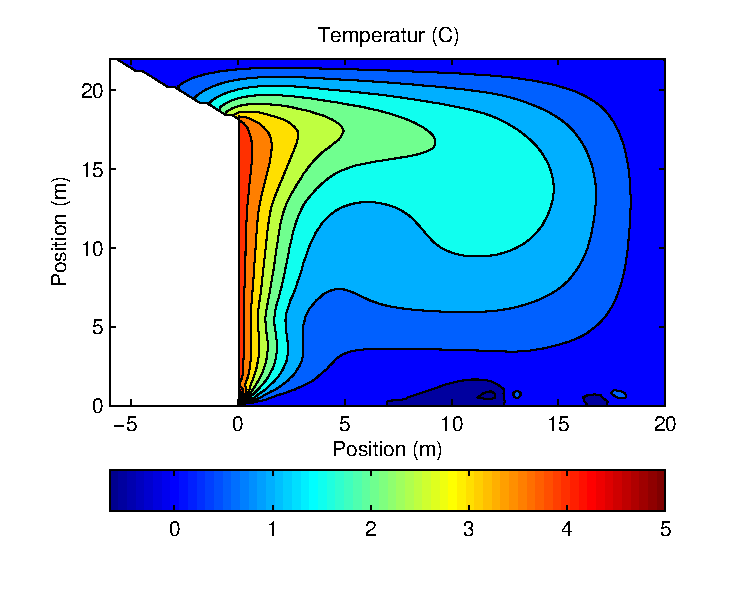
\includegraphics[width=10cm]{images/convectemperature.eps}
\caption{\label{fig:temp_dist}Temperaturfördelningen i $^\circ\mbox{C}$ utanför en vägg, beräknad med finita element av penaltymetoden. Inomhustempertur $\unit[20]{^\circ C}$, utomhustemperatur $\unit[0]{^\circ C}$.}
\end{figure}

% RESULTAT
Som kan ses i figuren \ref{fig:temp_dist} är luften närmast väggen upp till fem grader 
högre än omgivningen. När det blåser försvinner den här temperaturskillnaden. Detta 
visar tydligt hur viktigt det är att inte bara reglera efter utomhustemperaturen. 

%%%%%%%%%%%%%%%%%%%%%%%%%%%%%%%%%%%%%%%%%%%%

Även hastighetsfältet för temperaturens flöde, då det är vindstilla, har beräknats med finita element metoden 
applicerad på penaltymetoden. Detta kan ses i figur \ref{fig:velocityfield} där också 
beloppet av hastighetsfältet syns och det kan noteras att hastigheterna orimligt små.

\begin{figure}[hpbt]
\begin{center}
\subfloat[Hastighetsfält]{
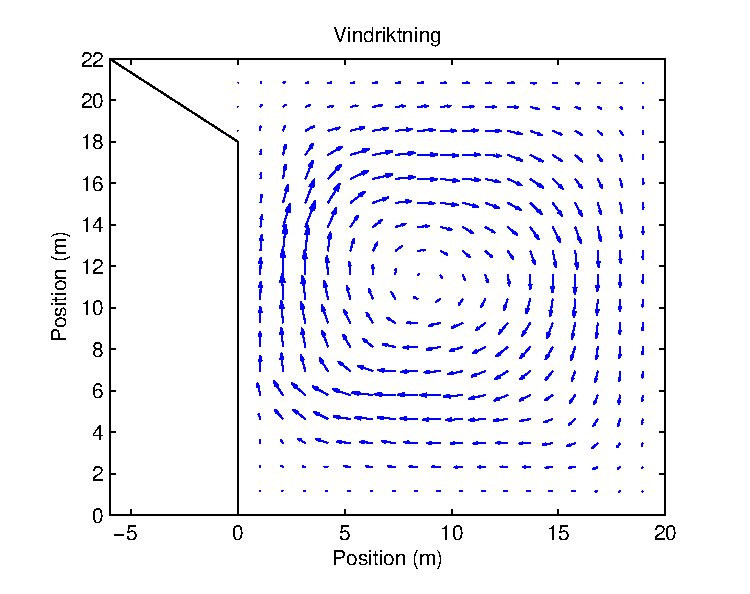
\includegraphics[scale=0.5]{images/convecquiver.eps}
}
\subfloat[Beloppet av hastigheten]{
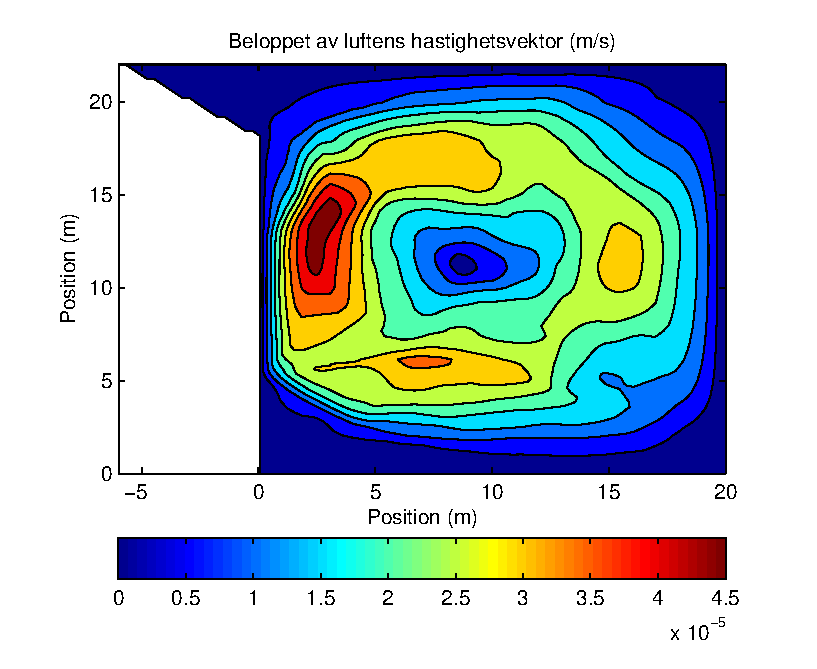
\includegraphics[scale=0.5]{images/convecspeed.eps}
}
\caption{\label{fig:velocityfield} Hur luften vid husväggen flödar vid en temperaturskillnad.}
\end{center}
\end{figure}

Då vi i sedan utifrån detta beräknar konvektionsparametern blir den därför väldigt liten, 
se figur \ref{fig:konv_param}. Tyvärr verkade det inte som att metodiken som användes 
för att framställa ovanstående data fungerade tillräckligt bra för att med någon 
noggrannhet studera fenomenet konvektion.  Vi menar dock att formen på hastighetsflödet intill marken och väggen
kan anses vara av rätt karaktär och visar på hur luften rör sig vid husväggen. Dock kan randerna mot
luft påverka då det ej var tillåtet för luften att passera de
kanterna. Detta kan också vara en felkälla till den absurt låga konvektionsparametern.


\begin{figure}[hpbt]
\centering
\subfloat[\label{fig:h_reftemp}Konvektionskoefficienten h mot referenstemperaturen]{
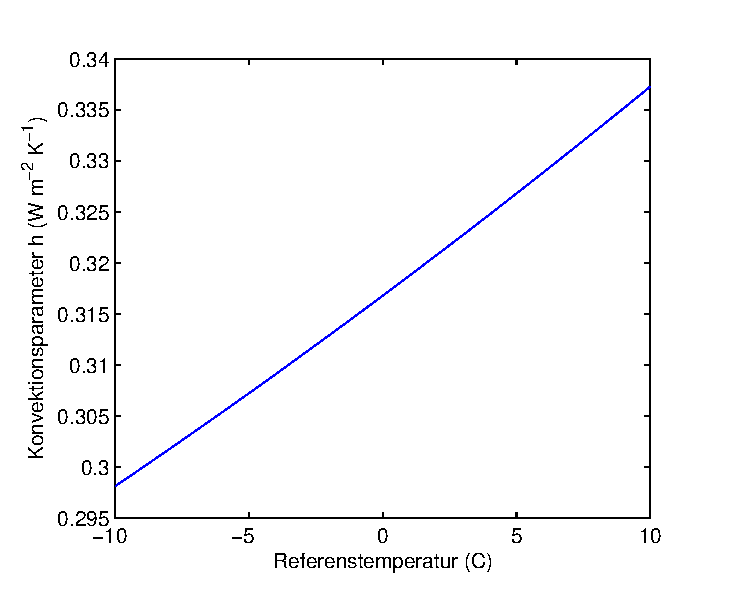
\includegraphics[scale=0.5]{images/convech.eps}
}
\subfloat[\label{fig:h_penalty}Konvektionskoefficienten h mot penaltyparametern]{
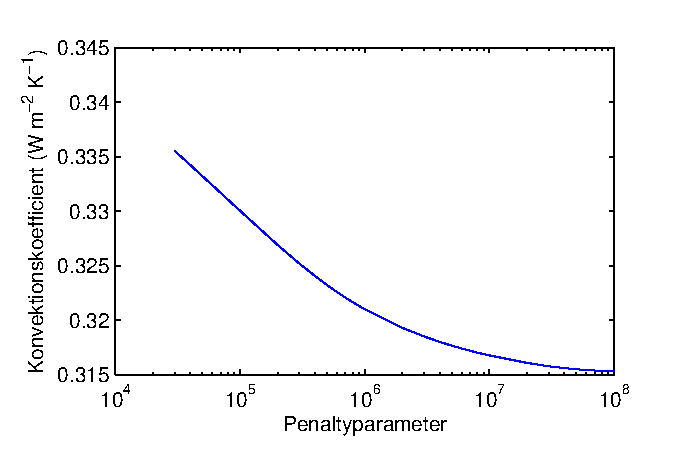
\includegraphics[scale=0.5]{images/convecpenalty.eps}
}\vspace{1cm}

\subfloat[\label{fig:h_volexp}Konvektionskoefficienten h mot den volymetriska expansionskoefficienten.]{
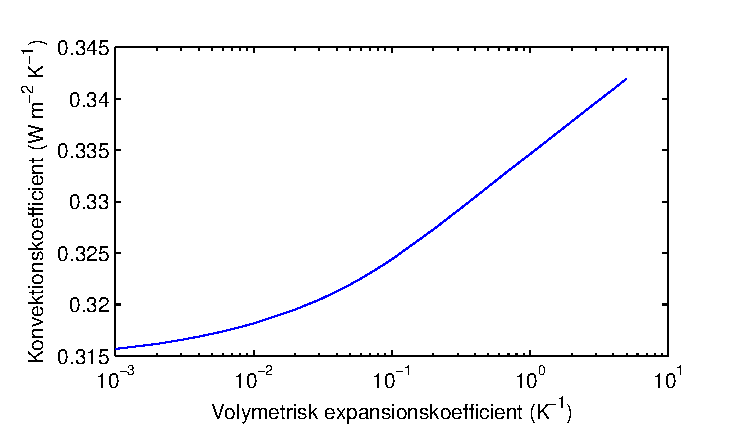
\includegraphics[scale=0.5]{images/convecbeta.eps}
}

\caption{\label{fig:konv_param}Stabilitetsberäkningar av konvektionskoefficienten h mot några
parametrar och naturkonstanter i finita elementsimuleringen av Navier-Stokes ekvationer.
Inomhustemperaturen är satt till konstanta $\unit[20]{^\circ C}$ med en vägg vars U-värde är
$\unit[1,18]{ Wm^{-2}K^{-1}}$. Detta skall motsvara söderväggen på fastigheten som detta arbete behandlar.}

\end{figure}

% RESULTAT
I figur \ref{fig:h_reftemp} har finita elementmodellens beteende studerats vid variation på några essentiella storheter i modellen.
Först har penaltyparametern varierats i figur \ref{fig:h_penalty} och här kan det ses att modellens beteende förändras inte nämnvärt
beroende på val av parameter när denna börjar vara i storleksordningen $\lambda = 10^7$. Det linjära förhållandet mellan
konvektionskoefficienten och temperaturdifferansen är intressant men saknar stöd i litteraturen då den rimligtvis borde vara
konstant eller nästan konstant. Slutligen varieras den volymetriska expansionskoefficienten
i figur \ref{fig:h_volexp}. Det är denna storhet
som gör att luften stiger när den blir varm och av denna anledning fenomenet fri konvektion uppstår. Konvektionskoefficienten
ser ut att öka mer än logaritmiskt men däremot ej så snabbt. Anledningen till att denna parameter varierades var för
att se hur stor den parametern skulle behöva bli innan konvektionen började få samma energitransporterande egenskaper
som den borde ha. Som kan ses så kommer inte modellen ens i närheten vid en väldigt stort vald volymetrisk expansionskoefficient.

